\documentclass[10pt,a4paper]{article}

\usepackage[utf8]{inputenc}
\usepackage{amsmath,amssymb}
\usepackage{geometry}
\usepackage{graphicx}
\usepackage{xcolor}
\usepackage{tikz}
\usetikzlibrary{shapes.geometric,calc,positioning}
\usepackage{fancyhdr}
\usepackage{hyperref}
\usepackage{array}
\usepackage{booktabs}
\usepackage{colortbl}

\geometry{
  a4paper,
  top=0.62in,
  bottom=0.62in,
  left=0.60in,
  right=0.60in,
  headheight=18pt,
  headsep=8pt,
  footskip=20pt
}

\setlength{\parindent}{0pt}
\setlength{\parskip}{4pt}

% --- Color Palette (Kurzgesagt / Quanta Magazine Inspired) ---
\definecolor{navybg}{HTML}{0B1325}
\definecolor{panelbg}{HTML}{0F172A}
\definecolor{slateink}{HTML}{1E293B}
\definecolor{mutedink}{HTML}{475569}

\definecolor{bubbleblue}{HTML}{2563EB}
\definecolor{bubblelight}{HTML}{EFF6FF}
\definecolor{bubbleborder}{HTML}{60A5FA}

\definecolor{insertgreen}{HTML}{16A34A}
\definecolor{insertlight}{HTML}{F0FDF4}
\definecolor{insertborder}{HTML}{4ADE80}

\definecolor{selectorange}{HTML}{EA580C}
\definecolor{selectlight}{HTML}{FFF7ED}
\definecolor{selectborder}{HTML}{FB923C}

\definecolor{frozenred}{HTML}{DC2626}
\definecolor{frozenlight}{HTML}{FEF2F2}
\definecolor{frozenborder}{HTML}{F87171}

\definecolor{purplecamp}{HTML}{7C3AED}
\definecolor{purplelight}{HTML}{F5F3FF}
\definecolor{purpleborder}{HTML}{A78BFA}

\definecolor{goldaccent}{HTML}{FACC15}
\definecolor{cyanaccent}{HTML}{38BDF8}
\definecolor{softgray}{HTML}{F8FAFC}
\definecolor{cardgray}{HTML}{F1F5F9}

\hypersetup{
  colorlinks=true,
  linkcolor=bubbleblue,
  citecolor=bubbleblue,
  urlcolor=bubbleblue
}

% --- Inline Jersey Badge Macro ---
\newcommand{\kidbadge}[2]{%
  \tikz[baseline=(char.base)]{%
    \node[
      shape=rectangle,
      rounded corners=2.5pt,
      fill=#1,
      text=white,
      inner xsep=4.5pt,
      inner ysep=1.5pt,
      font=\sffamily\bfseries\scriptsize
    ] (char) {#2};%
  }%
}

% --- Pretty Section Header Banner ---
\newcommand{\prettysection}[3]{%
  \vspace{3pt}%
  \noindent
  \begin{tikzpicture}
    \node[
      rectangle,
      rounded corners=4.5pt,
      fill=#2!10,
      draw=#2!60,
      line width=0.9pt,
      inner xsep=9pt,
      inner ysep=5pt,
      text width=\dimexpr\textwidth-20pt\relax,
      align=left
    ] (secbox) {%
      \tikz[baseline=(n.base)]{
        \node[circle, fill=#2, text=white, inner sep=2.2pt, font=\sffamily\bfseries\footnotesize] (n) {#1};
      }%
      \hspace{5pt}{\sffamily\bfseries\normalsize\color{navybg}#3}%
    };
    \fill[#2, rounded corners=1.5pt] (secbox.south west) rectangle ([xshift=3.8pt]secbox.north west);
  \end{tikzpicture}%
  \vspace{1pt}\par
}

% --- Styled Callout Card ---
\newcommand{\calloutcard}[5]{%
  \noindent
  \begin{tikzpicture}
    \node[
      rectangle,
      rounded corners=5pt,
      fill=#2,
      draw=#1!65,
      line width=1.0pt,
      inner xsep=10pt,
      inner ysep=7pt,
      text width=\dimexpr\textwidth-22pt\relax,
      align=left
    ] (card) {%
      {\sffamily\bfseries\scriptsize\tikz[baseline=(b.base)]{\node[rounded corners=2.5pt,fill=#1,text=white,inner xsep=5pt,inner ysep=1.6pt](b){#3};}}%
      \hspace{5pt}{\sffamily\bfseries\small\color{navybg}#4}\\[3pt]
      {\small\color{slateink}#5}%
    };
    \fill[#1, rounded corners=1.5pt] (card.south west) rectangle ([xshift=4pt]card.north west);
  \end{tikzpicture}\par
}

% --- Styled Figure Card with Height Control ---
\newcommand{\prettyfigure}[4]{%
  % #1 = max height, #2 = path, #3 = label, #4 = caption
  \noindent
  \begin{tikzpicture}
    \node[
      rectangle,
      rounded corners=6pt,
      fill=navybg,
      draw=cyanaccent!80,
      line width=1.1pt,
      inner sep=6pt,
      text width=\dimexpr\textwidth-14.4pt\relax,
      align=center
    ] (figcard) {%
      \includegraphics[width=0.985\textwidth,height=#1,keepaspectratio]{#2}\\[3pt]
      \begin{minipage}{0.96\textwidth}
        \raggedright
        {\sffamily\bfseries\scriptsize\color{goldaccent}#3}\hspace{3pt}%
        {\sffamily\scriptsize\color{white!92}#4}
      \end{minipage}
    };
  \end{tikzpicture}\par
}

% --- Header & Footer ---
\pagestyle{fancy}
\fancyhf{}
\renewcommand{\headrulewidth}{0pt}
\fancyhead[L]{{\sffamily\bfseries\scriptsize\color{mutedink}PROJECT DELPHI $\cdot$ YOUNG SCIENTIST'S ILLUSTRATED EDITION}}
\fancyhead[R]{{\sffamily\bfseries\scriptsize\color{bubbleblue}Self-Sorting Cells \& The ``Platonic Space'' Debate}}
\fancyfoot[L]{{\sffamily\scriptsize\color{mutedink}\texttt{github.com/fractastical/morpholib}}}
\fancyfoot[R]{%
  \tikz[baseline=(p.base)]{%
    \node[rounded corners=2.5pt, fill=navybg, text=goldaccent, font=\sffamily\bfseries\scriptsize, inner xsep=6pt, inner ysep=2pt] (p) {Page \thepage\ of 4};
  }%
}

\begin{document}
\color{slateink}

% ============================================================================
% PAGE 1: HERO BANNER + GYM CLASS PUZZLE + FIGURE 1
% ============================================================================
\noindent
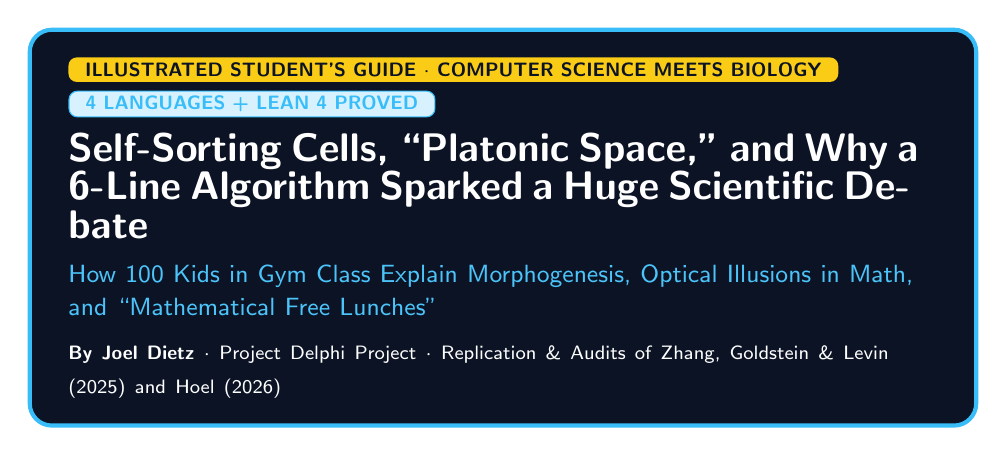
\begin{tikzpicture}
  \node[
    rectangle,
    rounded corners=8pt,
    fill=navybg,
    draw=cyanaccent,
    line width=1.5pt,
    inner xsep=14pt,
    inner ysep=10pt,
    text width=\dimexpr\textwidth-31pt\relax,
    align=left
  ] (hero) {%
    \tikz[baseline=(pill.base)]{
      \node[rounded corners=3pt, fill=goldaccent, text=navybg, font=\sffamily\bfseries\scriptsize, inner xsep=6pt, inner ysep=2pt] (pill) {ILLUSTRATED STUDENT'S GUIDE $\cdot$ COMPUTER SCIENCE MEETS BIOLOGY};
    }\hspace{5pt}%
    \tikz[baseline=(pill2.base)]{
      \node[rounded corners=3pt, fill=cyanaccent!20, draw=cyanaccent, text=cyanaccent, font=\sffamily\bfseries\scriptsize, inner xsep=6pt, inner ysep=1.8pt] (pill2) {4 LANGUAGES + LEAN 4 PROVED};
    }\\[5pt]
    {\sffamily\bfseries\Large\color{white}Self-Sorting Cells, ``Platonic Space,'' and Why a 6-Line Algorithm Sparked a Huge Scientific Debate}\\[4pt]
    {\sffamily\small\color{cyanaccent!90}How 100 Kids in Gym Class Explain Morphogenesis, Optical Illusions in Math, and ``Mathematical Free Lunches''}\\[4pt]
    {\sffamily\scriptsize\color{white!80}\textbf{By Joel Dietz} $\cdot$ Project Delphi Project $\cdot$ Replication \& Audits of Zhang, Goldstein \& Levin (2025) and Hoel (2026)}
  };
\end{tikzpicture}

\prettysection{1}{bubbleblue}{The Gym-Class Puzzle: What If There Is No Gym Teacher?}

{\small
Imagine \textbf{100 kids standing in a single line in gym class}, each wearing a sports jersey with a random number from \kidbadge{navybg}{\#1} to \kidbadge{navybg}{\#100}. Normally, the gym teacher (a \textbf{central controller}) walks up and down the line telling specific kids to trade places until everyone is lined up in order from $1$ to $100$.

In 2025, three scientists --- \textbf{Taining Zhang, Adam Goldstein, and Michael Levin} --- asked a fascinating question that connects computer science to how living embryos build bodies: \textbf{What if there is no gym teacher?} What if every kid is an independent ``cell'' who can only look at their neighbors and decide on their own whether to swap?
}

\calloutcard{bubbleblue}{softgray}{THE 3 ALGOTYPES}{Three Different ``Cell Personalities'' in the Same Line}{%
  \begin{itemize}\setlength{\itemsep}{2pt}\setlength{\topsep}{1pt}
    \item \kidbadge{bubbleblue}{Bubble Kids (B)} \textbf{The Neighbor Swappers:} Look only at the kid immediately to your left or right. If your jersey number is smaller than your left neighbor's (or bigger than your right neighbor's), trade places!
    \item \kidbadge{insertgreen}{Insertion Kids (I)} \textbf{The Careful Steppers:} Only step left if \emph{every single kid} to your left is already lined up in order.
    \item \kidbadge{selectorange}{Selection Kids (S)} \textbf{The Long-Range Teleporters:} Keep a mental finger pointing at slot $\#1$, then $\#2$, then $\#3\dots$ If your number is smaller than whoever is standing at that target slot, jump straight across the gym and swap with them!
  \end{itemize}
}

{\small
When they ran this simulation, they noticed \textbf{three wild behaviors}: \textbf{(1) Error Tolerance} (if a few \kidbadge{frozenred}{FROZEN \#99} kids refuse to move, the line still sorts around them); \textbf{(2) ``Delayed Gratification''} (the line sometimes looks \emph{messier} before getting cleaner); and \textbf{(3) ``Secret Clique Clustering''} (\kidbadge{bubbleblue}{B} kids group with \kidbadge{bubbleblue}{B} kids and \kidbadge{selectorange}{S} kids group with \kidbadge{selectorange}{S} kids, even though their jerseys hide their personality!).
}

\prettyfigure{0.37\textheight}{media/zhang_13yo_fig1_three_personalities.png}{ILLUSTRATED GUIDE 1:}{How the 3 personalities work --- and why Bubble gets blocked by \texttt{Frozen \#99}, Insertion needs a 3-line code rescue (\texttt{if FREEZE: prev = -1}), and Selection teleports right over the wall!}

\newpage

% ============================================================================
% PAGE 2: THE BIG DEBATE + DISCOVERY 1 + DISCOVERY 2 + FIGURE 2
% ============================================================================
\prettysection{2}{purplecamp}{The Big Debate: ``Platonic Ghost Minds'' vs.\ ``Nothing New Here!''}

{\small As soon as the paper came out, a big scientific argument broke out between two camps:}

\noindent
\begin{minipage}[t]{0.49\textwidth}
  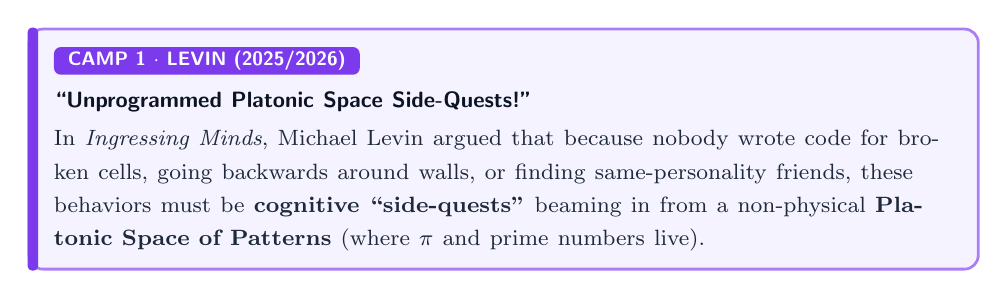
\begin{tikzpicture}
    \node[
      rectangle, rounded corners=5pt, fill=purplelight, draw=purplecamp!65, line width=1pt,
      inner xsep=9pt, inner ysep=6.5pt, text width=\dimexpr\textwidth-20pt\relax, align=left
    ] (c1) {%
      {\sffamily\bfseries\scriptsize\tikz[baseline=(b.base)]{\node[rounded corners=2.5pt,fill=purplecamp,text=white,inner xsep=5pt,inner ysep=1.5pt](b){CAMP 1 $\cdot$ LEVIN (2025/2026)};}}\\[3pt]
      {\sffamily\bfseries\footnotesize\color{navybg}``Unprogrammed Platonic Space Side-Quests!''}\\[2pt]
      {\footnotesize\color{slateink}In \emph{Ingressing Minds}, Michael Levin argued that because nobody wrote code for broken cells, going backwards around walls, or finding same-personality friends, these behaviors must be \textbf{cognitive ``side-quests''} beaming in from a non-physical \textbf{Platonic Space of Patterns} (where $\pi$ and prime numbers live).}
    };
    \fill[purplecamp, rounded corners=1.5pt] (c1.south west) rectangle ([xshift=3.8pt]c1.north west);
  \end{tikzpicture}
\end{minipage}\hfill
\begin{minipage}[t]{0.49\textwidth}
  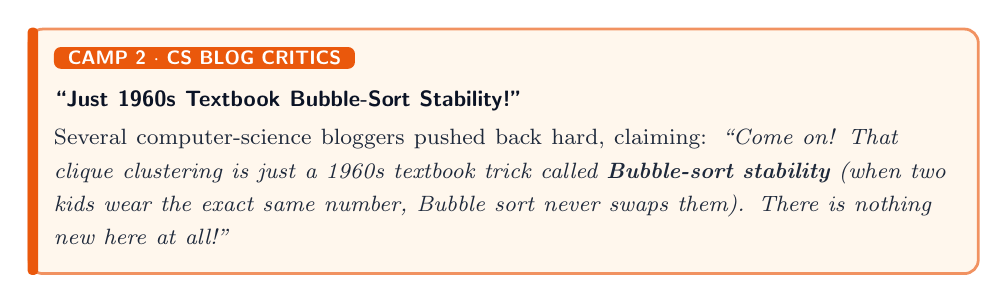
\begin{tikzpicture}
    \node[
      rectangle, rounded corners=5pt, fill=selectlight, draw=selectorange!65, line width=1pt,
      inner xsep=9pt, inner ysep=6.5pt, text width=\dimexpr\textwidth-20pt\relax, align=left
    ] (c2) {%
      {\sffamily\bfseries\scriptsize\tikz[baseline=(b.base)]{\node[rounded corners=2.5pt,fill=selectorange,text=white,inner xsep=5pt,inner ysep=1.5pt](b){CAMP 2 $\cdot$ CS BLOG CRITICS};}}\\[3pt]
      {\sffamily\bfseries\footnotesize\color{navybg}``Just 1960s Textbook Bubble-Sort Stability!''}\\[2pt]
      {\footnotesize\color{slateink}Several computer-science bloggers pushed back hard, claiming: \emph{``Come on! That clique clustering is just a 1960s textbook trick called \textbf{Bubble-sort stability} (when two kids wear the exact same number, Bubble sort never swaps them). There is nothing new here at all!''}\vspace{4pt}}
    };
    \fill[selectorange, rounded corners=1.5pt] (c2.south west) rectangle ([xshift=3.8pt]c2.north west);
  \end{tikzpicture}
\end{minipage}

{\small To find out who was right, we translated their original Python code into \textbf{C++20}, \textbf{JavaScript}, and the \textbf{Lean~4} math theorem prover, ran \textbf{3 ``what-if'' code surgery experiments}, and tested the system with \textbf{Erik Hoel's 2026 Causal Emergence 2.0} math. Turns out: \textbf{both camps got something right and something wrong!}}

\prettysection{3}{insertgreen}{Discovery \#1: The Sneaky 3-Line Code Rescue Inside Insertion Sort}

\calloutcard{insertgreen}{insertlight}{DISCOVERY \#1 $\cdot$ CODE SURGERY}{Did They Really Add ``Zero Code'' for Frozen Kids?}{%
  Levin wrote that they \emph{``did not add steps to the algorithm\dots\ to do specific things if an operation failed.''} For \kidbadge{bubbleblue}{Bubble (B)} kids, that's $100\%$ true! But \kidbadge{insertgreen}{Insertion (I)} kids have a strict rule: \emph{never move left unless everyone to your left is sorted}. If \kidbadge{frozenred}{FROZEN \#99} is stuck near the front of the line, the left side is \emph{never} sorted! When we checked lines 74--76 of \texttt{InsertionSortCell.py}, we found \textbf{3 lines of special code} (\texttt{if status == FREEZE: prev = -1}) that tell Insertion kids to reset their memory right after a frozen kid. When we deleted those 3 lines, Insertion Sort froze up and its error jumped $\mathbf{4.5\times}$ higher ($4.9 \to 21.95$)!
}

\prettysection{4}{frozenred}{Discovery \#2: Why ``Delayed Gratification'' Was an Optical Illusion of the Ruler!}

\prettyfigure{0.255\textheight}{media/zhang_13yo_fig2_two_rulers_illusion.png}{ILLUSTRATED GUIDE 2:}{Watch 4 kids swap $4 \leftrightarrow 1$ in $\mathbf{[2, 4, 1, 3] \to [2, 1, 4, 3]}$. Under \textbf{Ruler 1 (Total Out-of-Order Pairs $I$, green arches)}, messiness goes \textbf{STRICTLY DOWN ($3 \to 2$)}. Under \textbf{Ruler 2 (Neighbor Steps $E$, red arrows)}, it goes \textbf{UP ($1 \to 2$)} only because one big cliff ($4>1$) split into two small steps ($2>1$ and $4>3$)!}

\calloutcard{frozenred}{frozenlight}{DISCOVERY \#2 $\cdot$ HOEL'S CAUSAL EMERGENCE 2.0}{How Erik Hoel's 2026 Math Proves Which Ruler Is Real}{%
  \begin{itemize}\setlength{\itemsep}{1.5pt}\setlength{\topsep}{1pt}
    \item \textbf{Ruler 1 --- Total Out-of-Order Pairs $I(v)$ (Green Arches):} Counts \emph{every} pair of kids where a bigger number stands left of a smaller number. Every single Bubble swap reduces $I(v)$ by $\mathbf{-1}$ ($\mathbf{0}$ uphill steps out of 192 swaps!). In Erik Hoel's 2026 \emph{Causal Emergence 2.0} test, Ruler 1 is \textbf{$100\%$ deterministic with positive Causal Emergence ($\Delta\mathrm{CP} = +0.119$)}.
    \item \textbf{Ruler 2 --- Only Neighbor Steps $E(v)$ (Red Arrows):} Only looks at immediate neighbors. Because it throws away long-range pair information, it has \textbf{negative Causal Emergence ($\Delta\mathrm{CP} = -0.253$)}. Zero Bubble kids ever cross a wall --- Ruler 2 just had a blind spot!
  \end{itemize}
}

\newpage

% ============================================================================
% PAGE 3: DISCOVERY 3 (BLOG CRITICS WRONG TWICE) + FIGURE 3 + FIGURE 4
% ============================================================================
\prettysection{5}{selectorange}{Discovery \#3: Why the Computer-Science Blog Critics Were Wrong Twice!}

{\small Remember how the online blog critics claimed: \emph{``The Bubble and Selection kids only cluster together because of textbook Bubble-sort stability on duplicate numbers!''}? Our experiments proved the critics wrong \textbf{two different ways}:}

\calloutcard{selectorange}{selectlight}{DISCOVERY \#3 $\cdot$ TRAFFIC WAVES \& THE $C=2$ SMOKING GUN}{Sports Cars vs.\ Pedestrians --- Plus ``Anti-Clustering'' at $C = 2$!}{%
  \begin{enumerate}\setlength{\itemsep}{2pt}\setlength{\topsep}{1pt}
    \item \textbf{Proof 1 --- Zero Duplicate Numbers ($1 \dots 80$, All Unique):} When every kid wears a different number, ``duplicate-key stability'' is impossible because there are zero duplicates! Yet halfway through sorting, \kidbadge{bubbleblue}{B} and \kidbadge{selectorange}{S} kids \textbf{still cluster together ($0.50 \to 0.624$)}! Why? Because \kidbadge{selectorange}{Selection (S)} kids move like \textbf{sports cars} (teleporting small numbers straight to the front of the line) while \kidbadge{bubbleblue}{Bubble (B)} kids move like \textbf{pedestrians}, shoving a wave of Bubble kids into the right half of the gym!
    \item \textbf{Proof 2 --- The $C = 2$ ``Anti-Clustering'' Smoking Gun on Duplicate Numbers:} If textbook Bubble-sort stability merely preserved the starting random order of equal numbers, clustering would stay flat at $\mathbf{0.50}$ (random) for every group size $C$. Instead, because Selection kids always scan from the left ($0, 1, 2\dots$), \textbf{$75\%$ of Selection kids grab the LEFT half of every number's group (\texttt{S...S | B...B})}:
    \begin{itemize}\setlength{\itemsep}{1pt}\setlength{\topsep}{1pt}
      \item With $\mathbf{C = 2}$ \textbf{copies per number}, putting \texttt{S} on the left and \texttt{B} on the right of each pair creates $\mathtt{S\,B \mid S\,B \mid S\,B}$, driving clustering \textbf{BELOW random ($0.477 < 0.50$, Anti-Clustering!)}!
      \item With $\mathbf{C = 8\text{--}10}$ \textbf{copies per number}, each group forms $\mathtt{SSSSS \mid BBBBB}$, driving clustering \textbf{way UP to $0.659$}!
    \end{itemize}
  \end{enumerate}
}

\prettyfigure{0.242\textheight}{media/zhang_13yo_fig3_sports_cars_vs_pedestrians.png}{ILLUSTRATED GUIDE 3:}{Why Selection (\texttt{S}, orange) packs into the left half of each number's group and pushes Bubble (\texttt{B}, blue) into the right half --- creating $\mathtt{S\,B \mid S\,B \mid S\,B}$ \textbf{Anti-Clustering ($0.477 < 0.50$)} when $C=2$ (top) and $\mathtt{SSSS \mid BBBB}$ \textbf{Big Cliques ($0.659$)} when $C=8\text{--}10$ (bottom)!}

\prettyfigure{0.232\textheight}{media/zhang_13yo_fig4_real_data_curves.png}{ILLUSTRATED GUIDE 4:}{The real computer simulation curves! \textbf{Left (A):} Ruler 1 ($I(v)$, green) slides smoothly downhill with $0$ bumps while Ruler 2 ($E(v)$, red) has $47$ illusory bumps. \textbf{Right (B):} Across duplicate copies $C$, clustering dips below $0.50$ at $C=2$ ($0.477$) before climbing to $0.659$ at $C=10$ --- refuting the flat $0.50$ blog-critic prediction!}

\newpage

% ============================================================================
% PAGE 4: THE FINAL SCOREBOARD + TAKE-HOME LESSONS + FULL DATA REFERENCE
% ============================================================================
\prettysection{6}{bubbleblue}{The Final Scoreboard: Who Got What Right?}

\noindent
\renewcommand{\arraystretch}{1.32}
\begin{tabular}{>{\raggedright\arraybackslash\sffamily\bfseries\scriptsize\color{navybg}}p{0.19\textwidth} >{\raggedright\arraybackslash\scriptsize\color{slateink}}p{0.23\textwidth} >{\raggedright\arraybackslash\scriptsize\color{slateink}}p{0.22\textwidth} >{\raggedright\arraybackslash\scriptsize\color{slateink}}p{0.27\textwidth}}
  \rowcolor{navybg}
  \textcolor{goldaccent}{\sffamily\bfseries Mystery / Claim} &
  \textcolor{cyanaccent}{\sffamily\bfseries Camp 1 (Levin's Platonic Claim)} &
  \textcolor{selectborder}{\sffamily\bfseries Camp 2 (CS Blog Critics)} &
  \textcolor{insertborder}{\sffamily\bfseries What Our Code \& Math Audit Proved} \\
  \rowcolor{softgray}
  1.\ Sorting Around Frozen Kids &
  ``Zero special code was added for broken cells!'' &
  \emph{(Did not check the source code)} &
  \textbf{True for Bubble \& Selection}, but \textbf{Insertion Sort has 3 lines of reset code} (\texttt{if FREEZE: prev = -1})! \\
  \rowcolor{cardgray}
  2.\ ``Delayed Gratification'' (Messiness Going Up) &
  ``Cells temporarily de-sort to walk around a barrier!'' &
  \emph{(Did not test the ruler)} &
  \textbf{Optical illusion of Ruler 2 ($E$)!} Zero Bubble kids cross a barrier, and \textbf{Ruler 1 ($I$) goes strictly downhill ($\Delta I = -1$)} on every swap! \\
  \rowcolor{softgray}
  3.\ Clique Clustering (All Unique Numbers) &
  ``An unprogrammed social side-quest!'' &
  ``Impossible without duplicate numbers!'' &
  \textbf{Critics wrong!} Clustering still hits $\mathbf{0.624}$ because Selection ``sports cars'' outrun Bubble ``pedestrians''! \\
  \rowcolor{cardgray}
  4.\ Clique Clustering (Duplicate Numbers) &
  ``Cells seek out same-personality neighbors!'' &
  ``Just 1960s textbook Bubble-sort stability!'' &
  \textbf{Critics wrong again!} Selection grabs the left half (\texttt{S...S|B...B}), causing \textbf{Anti-Clustering ($0.477 < 0.50$) at $C=2$} and \textbf{Cliques ($0.659$) at $C=10$}! \\
\end{tabular}

\calloutcard{insertgreen}{insertlight}{THE BIG TAKEAWAY $\cdot$ WHY BOTH BIOLOGY AND MATH WIN}{What Are ``Mathematical Free Lunches'' in Living Things?}{%
  \begin{enumerate}\setlength{\itemsep}{2pt}\setlength{\topsep}{1pt}
    \item \textbf{What Michael Levin Got Right (Mathematical ``Free Lunches''):}
    You really \emph{do} get ``more out than you put in'' when living cells follow simple local rules! Without any central gym teacher or friend-detector code, the geometry of permutations and differences in movement speed automatically give embryos self-sorting, error resistance, and group separation for free.
    \item \textbf{What Erik Hoel's Causal Emergence 2.0 Taught Us:}
    Sometimes a system looks spooky or chaotic only because we are measuring it with a blurry ruler! When we switch from Neighbor Steps $E(v)$ ($\Delta\mathrm{CP} = -0.253$) to Total Out-of-Order Pairs $I(v)$ ($\Delta\mathrm{CP} = +0.119$), the mystery vanishes and the macro-law becomes $\mathbf{100\%}$ \textbf{deterministic}.
    \item \textbf{Why Checking the Actual Code Always Matters:}
    By reading all 6 lines of cell rules, testing them across \textbf{Python, C++20, JavaScript, and Lean~4}, and sweeping $C = 2 \dots 10$ copies per number, we uncovered both the 3-line \texttt{prev = -1} rescue in Insertion Sort and the $C=2$ Anti-Clustering dip that neither camp had noticed!
  \end{enumerate}
}

\prettyfigure{0.34\textheight}{media/zhang_hoel_quantifying_emergence_ce2.png}{BONUS RESEARCH LAB DASHBOARD:}{The full 4-panel research figure from our technical paper showing Hoel's Causal Emergence 2.0 ($\Delta\mathrm{CP} = +0.1191$ on $I(v)$ vs.\ $-0.2525$ on $E(v)$), why CE 2.0 beats CE 1.0, and the exact $C=2$ anti-clustering law!}

\end{document}
